\medskip

\textbf{Partie A}

\smallskip

\begin{enumerate}
	\item $f$ est dérivable sur son ensemble de définition, en tant que fraction rationnelle.

$\begin{aligned}[t] \forall x \in [0~;~1],\quad f'(x) &= \dfrac{0,96 \times (0,93 x + 0,03) - (0,96x \times 0,93)}{(0,93x + 0,03)^2}\\
&=\dfrac{0,8928 x + 0,0288 - 0,8928 x}{(0,93x + 0,03)^2}\\
&=\dfrac{0,0288}{(0,93x + 0,03)^2}\end{aligned}$

On arrive donc bien à l'expression demandée.

	\item On a une fonction dérivée qui est le quotient d'un numérateur strictement positif par un dénominateur qui est le carré d'un réel non nul, donc strictement positif également, donc pour tout $x$ dans $ [0~;~1] $, $f'(x)$ est strictement positif.

On en déduit que la fonction $f$ est strictement croissante sur $ [0~;~1] $.
	\end{enumerate}

	\bigskip

	\textbf{Partie B}

	\smallskip

	\begin{enumerate}
		\item On a l'arbre suivant :

		\begin{center}
			\hfill~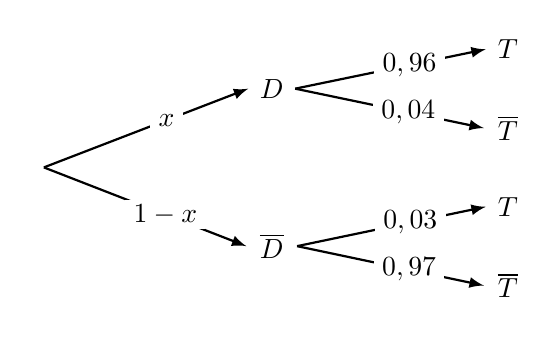
\begin{tikzpicture}[xscale=1,yscale=1,baseline={(R.base)}]
				
				\tikzstyle{fleche}=[->,>=latex,thick]
				\tikzstyle{noeud}=[fill=white,circle,inner sep=2pt]
				\tikzstyle{feuille}=[fill=white,circle,inner sep=2pt]
				\tikzstyle{etiquette}=[pos=0.6,fill=white, inner xsep=3pt, inner ysep=1.5pt]
				
				\def\DistanceInterNiveaux{3}
				\def\DistanceInterFeuilles{1}
				
				\def\NiveauA{(0)*\DistanceInterNiveaux}
				\def\NiveauB{(1)*\DistanceInterNiveaux}
				\def\NiveauC{(2)*\DistanceInterNiveaux}
				\def\InterFeuilles{(-1)*\DistanceInterFeuilles}
				
				\node[noeud] (R) at ({\NiveauA},{(1.5)*\InterFeuilles}) {};
				\node[noeud] (Ra) at ({\NiveauB},{(0.5)*\InterFeuilles})            {$D$};
				\node[feuille] (Raa) at ({\NiveauC},{(0)*\InterFeuilles})           {$T$};
				\node[feuille] (Rab) at ({\NiveauC},{(1)*\InterFeuilles}) {$\overline{T}$};
				\node[noeud] (Rb) at ({\NiveauB},{(2.5)*\InterFeuilles})  {$\overline{D}$};
				\node[feuille] (Rba) at ({\NiveauC},{(2)*\InterFeuilles})           {$T$};
				\node[feuille] (Rbb) at ({\NiveauC},{(3)*\InterFeuilles}) {$\overline{T}$};
				
				\draw[fleche] (R.east)--(Ra.west) node[etiquette]   {$x$};
				\draw[fleche] (Ra.east)--(Raa.west) node[etiquette] {$0,96$};
				\draw[fleche] (Ra.east)--(Rab.west) node[etiquette] {$0,04$};
				\draw[fleche] (R.east)--(Rb.west) node[etiquette]   {$1 - x$};
				\draw[fleche] (Rb.east)--(Rba.west) node[etiquette] {$0,03$};
				\draw[fleche] (Rb.east)--(Rbb.west) node[etiquette] {$0,97$};
			\end{tikzpicture} \hfill~	\end{center}

		\item Ici, on nous demande de déterminer :\quad $P(D \cap T)$

		$P(\mathrm{D} \cap \mathrm{T}) = P(D)\times P_D(T) = x \times 0,96 = 0,96x$.

		\item Les évènements $D$ et $\overline{D}$ partitionnent l'univers, donc, d'après la loi des probabilités totales, on a :

$\begin{aligned} P(T) &= P(D \cap T) + P(\overline{D} \cap T)\\
&= 0,96x + (1 - x) \times 0,03\\
&= 0,96x + 0,03 - 0,03x\\
&= 0,93x + 0,03\end{aligned}$

On arrive bien à la probabilité annoncée.

		\item Dans cette question, on veut calculer $P_T(D)$.

Par définition des probabilités conditionnelles, on a :\quad $P_T(D) = \dfrac{P(D \cap T)}{P(T)}$.

D'après les questions précédentes, cela donne :\quad $P_T(D) = \dfrac{0,96x}{0,93x + 0,03} = f(x)$.

On est, dans cette question, avec 50 sportifs dopés sur les \np{1000} testés, donc en choisissant un sportif au hasard, on est en situation d'équiprobabilité et donc la probabilité qu'un sportif soit dopé est, pour cette question $x = \dfrac{50}{\np{1000}} = 0,05$.

La probabilité demandée est donc bien $f(0,05) = \dfrac{0,96 \times 0,05}{0,93\times 0,05 + 0,03} = \dfrac{32}{51}\approx 0,627$ soit environ 0,63 au centième près.

		\item \begin{enumerate}
			\item La valeur prédictive positive du test est donc la probabilité $P_T(D)$. D'après la question \textbf{4. a.}, pour toute probabilité $x$ dans $ [0~;~1] $, on a :\quad $P_T(D)= f(x)$.

On veut donc résoudre, dans $ [0~;~1] $, l'inéquation :\quad $f(x) \geqslant 0,9$.

$\begin{aligned} f(x) \geqslant 0,9&\iff \dfrac{0,96x}{0,93x + 0,03 } \geqslant 0,9\\
&\iff 0,96x \geqslant 0,9 (0,93x+0,03) \quad \text{car sur } [0~;~1],\quad 0,93x + 0,03 >0\\
&\iff (0,96 - 0,9\times 0,93)x \geqslant 0,9\times 0,03\\
&\iff 0,123x \geqslant 0,027\\
&\iff x \geqslant \dfrac{27}{123}	=\dfrac{9}{41 }	\end{aligned} $

C'est donc pour $x$ supérieur à $ \dfrac{9}{41} \approx 0,22$ que la valeur prédictive positive du test sera supérieure ou égale à 0,9.

\item Si on accepte comme vraie l'affirmation \og les sportifs les plus performants [sont les] plus fréquemment dopés\fg{}, alors le fait de restreindre la population testée aux sportifs les plus performants doit avoir pour conséquence de faire augmenter $x$, la proportion de sportifs dopés dans la population testée.

Comme la valeur prédictive positive est donnée par $f(x)$ et que la fonction $f$ est strictement croissante sur $ [0~;~1] $, plus $x$ augmente, plus $f(x)$ augmente et donc plus on teste une population où la proportion de dopés est élevée (ce qui est le cas si on ne teste que les sportifs les plus performants), meilleure est la valeur prédictive positive du test.
		\end{enumerate}
	\end{enumerate}

\vspace{5mm}
